\chapter{Realization}
\minitoc
\newpage

\setcounter{secnumdepth}{0} % Set the section counter to 0 so next section is not counted in toc
% ----------------------- Introduction ----------------------- %
\section{Introduction}
A project can always look simple from the outside, however if we dive deeply into how most software is made, we can see that it's not that simple of a process.
Therefore, this chapter will list all of the technologies that we've used and also some of the major technical difficulties we've come in contact with during the realization of our project.

\setcounter{secnumdepth}{2} % Resume counting the sections for the toc with a depth of 2 (Sections and sub-sections)
% ----------------------------------- SECTIONS (v) ----------------------------------- %
% ----------------------- Deployment process ----------------------- %
\section{Deployment process}
We will now explain the approach we adopted to continuously integrate, deploy and deliver our application as per the best practices of DevOps previously mentioned in \textbf{Chapter 3: State of the art}.
The deployment is currently supported on two different environments; the staging environment where we make sure our application works as intended, and of course the production environment.

% ----------------------- Technologies ----------------------- %
\section{Technologies}
This part is reserved for the presentation of all of the software used in the realization of the project and includes but is not limited to; programming languages, frameworks, technologies, etc...

\medskip
For a comparative analysis on some of our choices, see \textbf {Chapter 2: State of the art}.

\begin{itemize}
    \item \textbf{Kubernetes:} \newline The most powerful tool for managing containerized workloads in the cloud. \newline
          \begin{minipage}{\linewidth}
              \centering
              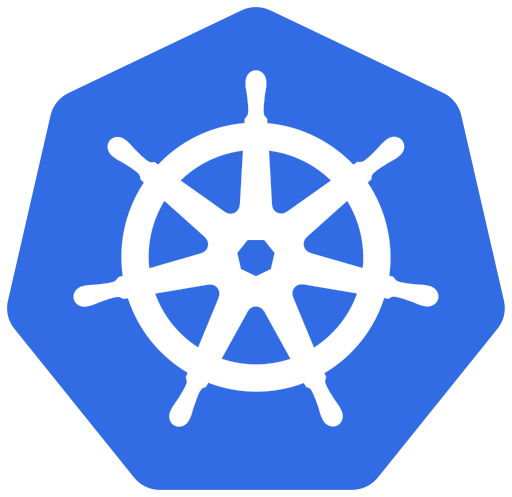
\includegraphics[width=3.5cm]{src/assets/logos/kubernetes_512x512.png}
              \captionof{figure}{Logo of Kubernetes}
          \end{minipage}

          \newpage
    \item \textbf{Squid Proxy:} \newline \cite{squid} Squid is a caching proxy for the Web that supports HTTP, HTTPS, FTP and more. \newline
          \begin{minipage}{\linewidth}
              \centering
              
\includegraphics[width=6cm]{src/assets/logos/squid-proxy.png}
              \captionof{figure}{Logo of Squid Proxy}
          \end{minipage}
    \item \textbf{LaTeX:} \newline \cite{latex-project} A high-quality document preparation and typesetting system for technical grade documents. \newline \newline
          \begin{minipage}{\linewidth}
              \centering
              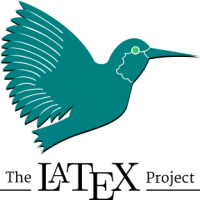
\includegraphics[width=4cm]{src/assets/logos/latex_200x200.png}
              \captionof{figure}{Logo of The LaTeX Project}
          \end{minipage}

          \newpage
\end{itemize}

% ----------------------- Difficulties encountered ----------------------- %
\section{Difficulties encountered}
\subsection{Stateful Kubernetes}
One issue we had is data persistence in Kubernetes.
Kubernetes is -by design- used for stateless applications.
However, since we're using an Elasticsearch database, we definitely needed a way to persist our data across system reboots or crashes.

\setcounter{secnumdepth}{0} % Set the section counter to 0 so next section is not counted in toc
% ----------------------- Conclusion ----------------------- %
\section{Conclusion}
In this chapter, we listed all of the technology stack that we used for our app as well as some of the most weighty issues we've encountered.
We also listed some our solutions for the ones we could solve following the best practices of software development.
